% Provenance (never printed): old seconde/premiere S material on the
% atmosphere (water vapour, saturation, cloud formation, the vertical motion
% of air) and enseignement scientifique premiere (water cycle); see
% sources/book2/PROVENANCE.md. Every saturation value, lapse rate,
% condensation level and the lee-wind example are computed in
% figdata/grade-10/clouds.py from the IAPWS saturation curves; the soundings
% are invented examples, said so in the text.
\chapter{لماذا تتكون السحب}\label{ch:g10:why-clouds-form}

على شرفة في الصيف تقف كأس من الماء المثلج على طاولة. وفي غضون دقيقة تكسو جدارها
الخارجي قطرات دقيقة، وتنتشر حلقة من الماء عند قاعدتها. لم يتسرب الماء عبر الكأس:
بل خرج من الهواء، الذي برد حيث لامس الزجاج البارد. وبعد بضع ساعات، على ارتفاع
كيلومترات فوق السهل، يحدث الشيء نفسه على نطاق واسع: فقاعات من الهواء الدافئ
تصعد وتبرد، وعند ارتفاع معين يظهر الماء الذي تحمله على شكل أكوام بيضاء من السحب
مسطحة القاعدة تُسمى الركام. يشرح هذا الفصل كم من بخار الماء يستطيع الهواء أن
يحمل، ولماذا يبرد الهواء الصاعد، وعلى أي ارتفاع تتكون السحب، ولماذا تبقى مسطحة
في بعض الأيام وتتعالى في أيام أخرى حتى تصير عواصف رعدية، وكيف تتحول قطيرات السحاب
الدقيقة إلى مطر وثلج.

\begin{omfigure}
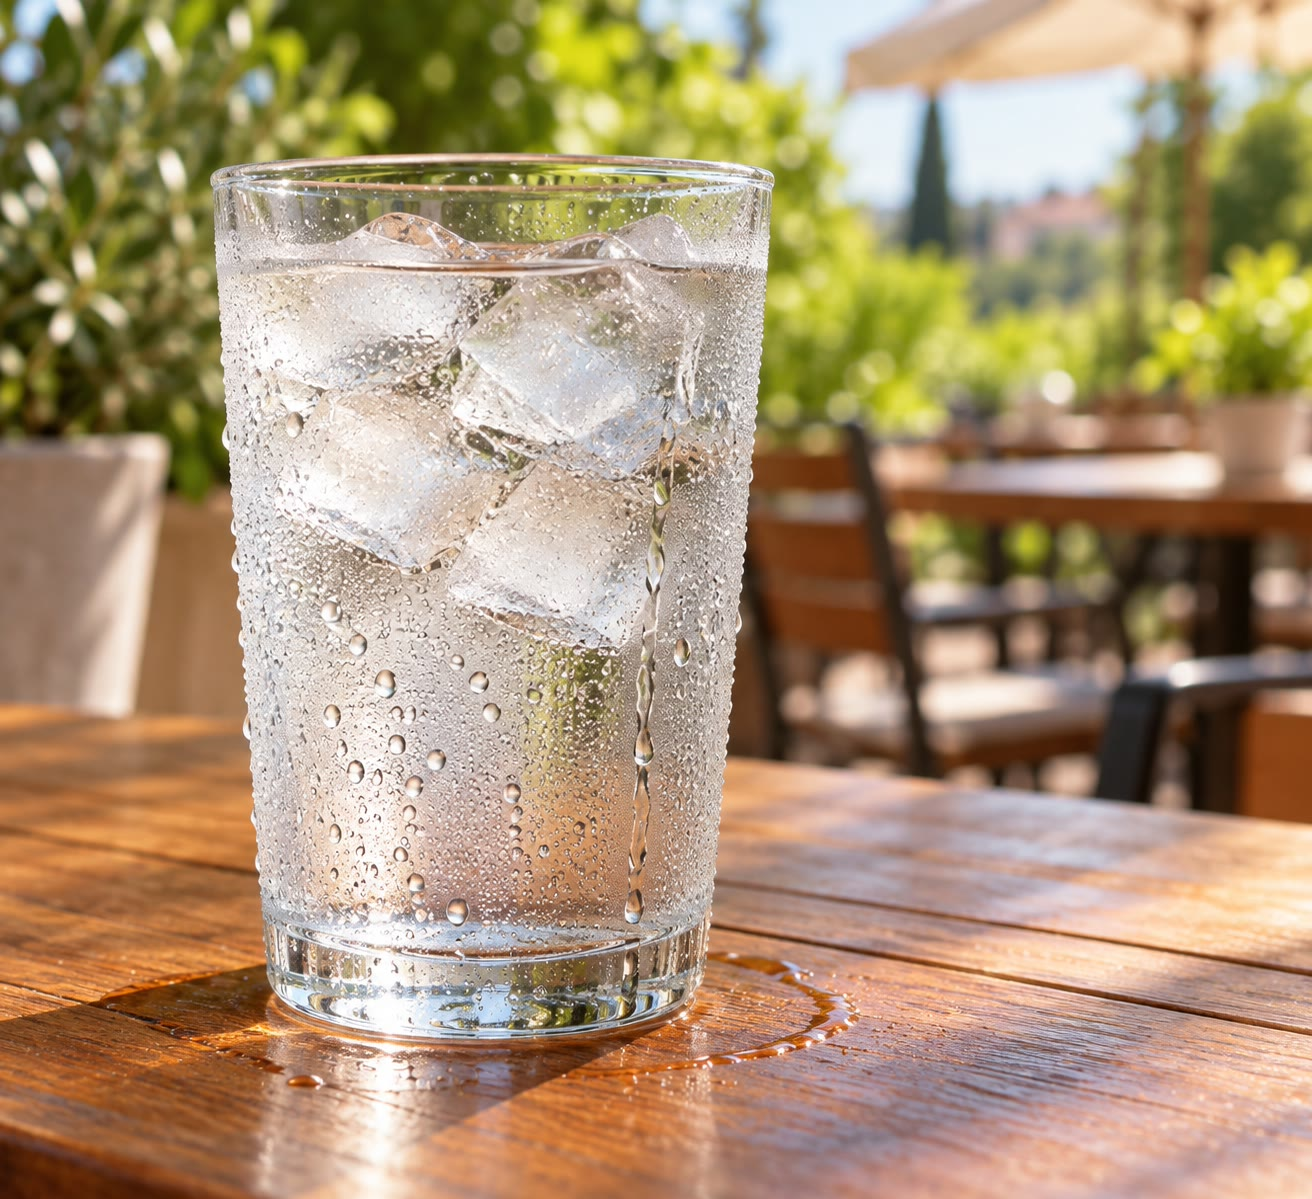
\includegraphics[width=0.5\linewidth]{images/book2/ai/g10-cold-glass.jpg}

{\small كأس من الماء المثلج على شرفة في الصيف: تتكون قطرات على جدارها الخارجي، حيث
يبرد الهواء الملامس للزجاج.}
\end{omfigure}

\begin{recall}
تتكون السحب من قطيرات ماء دقيقة أو بلورات جليد؛ وتُصنَّف في عائلات بحسب شكلها
وارتفاعها، وتعطي المطر والثلج والبَرَد، التي تُقاس بمقياس المطر (الكتاب 1، الصف
4). وتنخفض درجة حرارة الهواء مع الارتفاع عبر الطبقة الدنيا من الغلاف الجوي، بنحو
\qty{6.5}{\degreeCelsius} لكل كيلومتر في المتوسط؛ وهذا هو معدل التناقص الحراري
البيئي، والجبهات تفصل بين كتل هوائية مختلفة الحرارة (الكتاب 1، الصف 8). وينخفض
الضغط مع الارتفاع (كتب الفيزياء). ويتبخر الماء ويتكاثف، والتبخر يمتص \omterm{def:g10:earth-energy-budget:latent-heat}{حرارة كامنة}
يعيدها التكاثف (كتب الفيزياء و\cref{ch:g10:earth-energy-budget}).
\end{recall}
% ledger: nasa:grc-atmosphere

\section{بخار الماء والتشبع}

يحتوي الهواء دائمًا على قدر من بخار الماء، وهو غاز غير مرئي. وما يستطيع أن يحويه
منه يتوقف قبل كل شيء على درجة حرارته.

\begin{definition}[التشبع؛ الرطوبة النسبية]\label{def:g10:why-clouds-form:humidity}
يكون الهواء \emph{مشبعًا}\index{تشبع} حين يحتوي على أكبر كتلة من بخار الماء
يستطيع أن يحملها عند درجة حرارته، وهي \emph{محتواه عند
التشبع}؛ وكل بخار زائد يتكاثف قطيرات. و\emph{الرطوبة
النسبية}\index{رطوبة نسبية} للهواء هي محتواه من بخار الماء مقسومًا على محتواه
عند التشبع في درجة الحرارة نفسها والضغط نفسه، معبَّرًا عنها بنسبة مئوية.
\end{definition}

يُقاس محتوى الهواء من الماء هنا بغرامات البخار لكل كيلوغرام من الهواء الجاف
(\unit{g/kg}): فكتلة الهواء التي تصعد أو تهبط دون أن تكتسب ماء أو تفقده تحتفظ
بالمحتوى نفسه، حتى وهي تتمدد.

\begin{omfigure}
\begin{tikzpicture}
\begin{axis}[omrecord, width=0.88\linewidth, height=6.2cm, xmin=-10, xmax=40,
  ymin=0, ymax=50, xlabel={\foreignlanguage{arabic}{درجة الحرارة \babelsublr{(\unit{\degreeCelsius})}}},
  ylabel={\foreignlanguage{arabic}{المحتوى عند التشبع \babelsublr{(\unit{g/kg})}}}, xtick={-10,0,...,40},
  tick label style={font=\small}, label style={font=\small}]
\addplot[omDef!85!black, thick] table[x=T_C, y=ws_gkg] {figdata/out/grade-10-clouds-sat.dat};
\addplot[only marks, mark=*, mark size=1.8pt, omThm!85!black] coordinates {(28,11.37)};
\addplot[only marks, mark=o, mark size=1.8pt, omThm!85!black] coordinates {(16,11.37)};
\draw[->, omThm!85!black, thick] (axis cs:27.2,11.37) -- (axis cs:16.9,11.37);
\node[anchor=north, font=\footnotesize, omThm!85!black] at (axis cs:28,10.6) {\foreignlanguage{arabic}{هواء عند \babelsublr{\qty{28}{\degreeCelsius}}}};
\node[anchor=south east, font=\footnotesize, omThm!85!black] at (axis cs:15.5,12.2) {نقطة الندى};
\node[anchor=south east, font=\footnotesize, omDef!85!black, align=right] at (axis cs:31,34) {\foreignlanguage{arabic}{فوق المنحنى:}\\يتكاثف البخار};
\node[anchor=south west, font=\footnotesize, omDef!85!black] at (axis cs:31,2.5) {غير مشبع};
\node[anchor=north west, font=\footnotesize, omDef!85!black] at (axis cs:34,31.5) {التشبع};
\end{axis}
\end{tikzpicture}

{\small أكبر كتلة من بخار الماء يستطيع كيلوغرام من الهواء أن يحملها، بحسب درجة
الحرارة، عند ضغط مستوى سطح البحر (فوق الماء السائل؛ محسوبة من المعيار الدولي
للماء). فالهواء عند \qty{28}{\degreeCelsius} الذي يحمل \qty{11.4}{g/kg} (النقطة)
بعيد عن \omterm{def:g10:why-clouds-form:humidity}{التشبع}؛ وإذا بُرّد دون أن يفقد ماء، صار \omterm{def:g10:why-clouds-form:humidity}{مشبعًا} عند
\qty{16}{\degreeCelsius} (الدائرة).}
\end{omfigure}
% ledger: iapws:vapour-pressure, ciaaw:abridged-2024, earth:Mmol, const:R (computed in figdata/grade-10/clouds.py)

يصعد المنحنى بشدة: \qty{3.8}{g/kg} عند \qty{0}{\degreeCelsius}،
و\qty{14.7}{g/kg} عند \qty{20}{\degreeCelsius}، و\qty{27.2}{g/kg} عند
\qty{30}{\degreeCelsius}. فكل احترار بمقدار \qty{10}{\degreeCelsius} يضاعف
تقريبًا الماء الذي يستطيع الهواء أن يحمله. ولهذا يستطيع الهواء المداري أن يحمل
أمطارًا غزيرة، ولهذا لا يحمل هواء الشتاء القطبي، حتى وهو \omterm{def:g10:why-clouds-form:humidity}{مشبع}، شيئًا
يُذكر.

\begin{definition}[نقطة الندى]\label{def:g10:why-clouds-form:dew-point}
\emph{نقطة الندى}\index{نقطة الندى} للهواء هي درجة الحرارة التي يجب أن يُبرَّد
إليها، مع المحافظة على محتواه من الماء وعلى ضغطه، كي يصير
\omterm{def:g10:why-clouds-form:humidity}{مشبعًا}.
\end{definition}

\begin{method}[الرطوبة النسبية ونقطة الندى من جدول]\label{met:g10:why-clouds-form:table}
\begin{enumerate}
  \item اقرأ في الجدول المحتوى عند \omterm{def:g10:why-clouds-form:humidity}{التشبع} عند درجة حرارة الهواء.
  \item \omterm{def:g10:why-clouds-form:humidity}{الرطوبة النسبية}: اقسم محتوى الهواء من الماء عليه.
  \item \omterm{def:g10:why-clouds-form:dew-point}{نقطة الندى}: ابحث في الجدول عن درجة الحرارة التي يساوي المحتوى عند
        \omterm{def:g10:why-clouds-form:humidity}{التشبع} فيها محتوى الهواء من الماء.
\end{enumerate}
\end{method}

\begin{example}[صباح صيفي]\label{ex:g10:why-clouds-form:morning}
% ledger: iapws:vapour-pressure (values computed in figdata/grade-10/clouds.py)
عند \qty{20}{\degreeCelsius} يحتوي الهواء على \qty{11.4}{g/kg}. والمحتوى عند
\omterm{def:g10:why-clouds-form:humidity}{التشبع} عند \qty{20}{\degreeCelsius} هو \qty{14.7}{g/kg}، \omterm{def:g10:why-clouds-form:humidity}{فالرطوبة النسبية}
$11.4/14.7 \approx \qty{78}{\percent}$. ويكون المحتوى عند \omterm{def:g10:why-clouds-form:humidity}{التشبع}
\qty{11.4}{g/kg} عند \qty{16}{\degreeCelsius}: فتلك هي \omterm{def:g10:why-clouds-form:dew-point}{نقطة
الندى}. وبعد الظهر، يكون للهواء نفسه وقد سخن إلى \qty{28}{\degreeCelsius}
(محتواه عند \omterm{def:g10:why-clouds-form:humidity}{التشبع} \qty{24.1}{g/kg}) \omterm{def:g10:why-clouds-form:humidity}{رطوبة نسبية} لا تتجاوز
\qty{47}{\percent} --- مع أن فيه الماء نفسه تمامًا.
\end{example}

الكأس في المشهد الافتتاحي أبرد من \omterm{def:g10:why-clouds-form:dew-point}{نقطة ندى} الهواء المحيط بها: فالهواء الملامس لها
يبرد إلى ما دون \omterm{def:g10:why-clouds-form:dew-point}{نقطة نداه} فيترك ماء على الزجاج. وفي ليلة صافية، يفقد العشب وأسطح
السيارات حرارة بإشعاع أشعة تحت حمراء نحو السماء فتصير أبرد من الهواء: فيتكون عليها
الندى، أو الصقيع دون \qty{0}{\degreeCelsius}. وحين تبرد طبقة كاملة من الهواء
قرب الأرض إلى \omterm{def:g10:why-clouds-form:dew-point}{نقطة نداها}، تتكون قطيرات في الهواء نفسه: إنه الضباب.

\begin{omfigure}
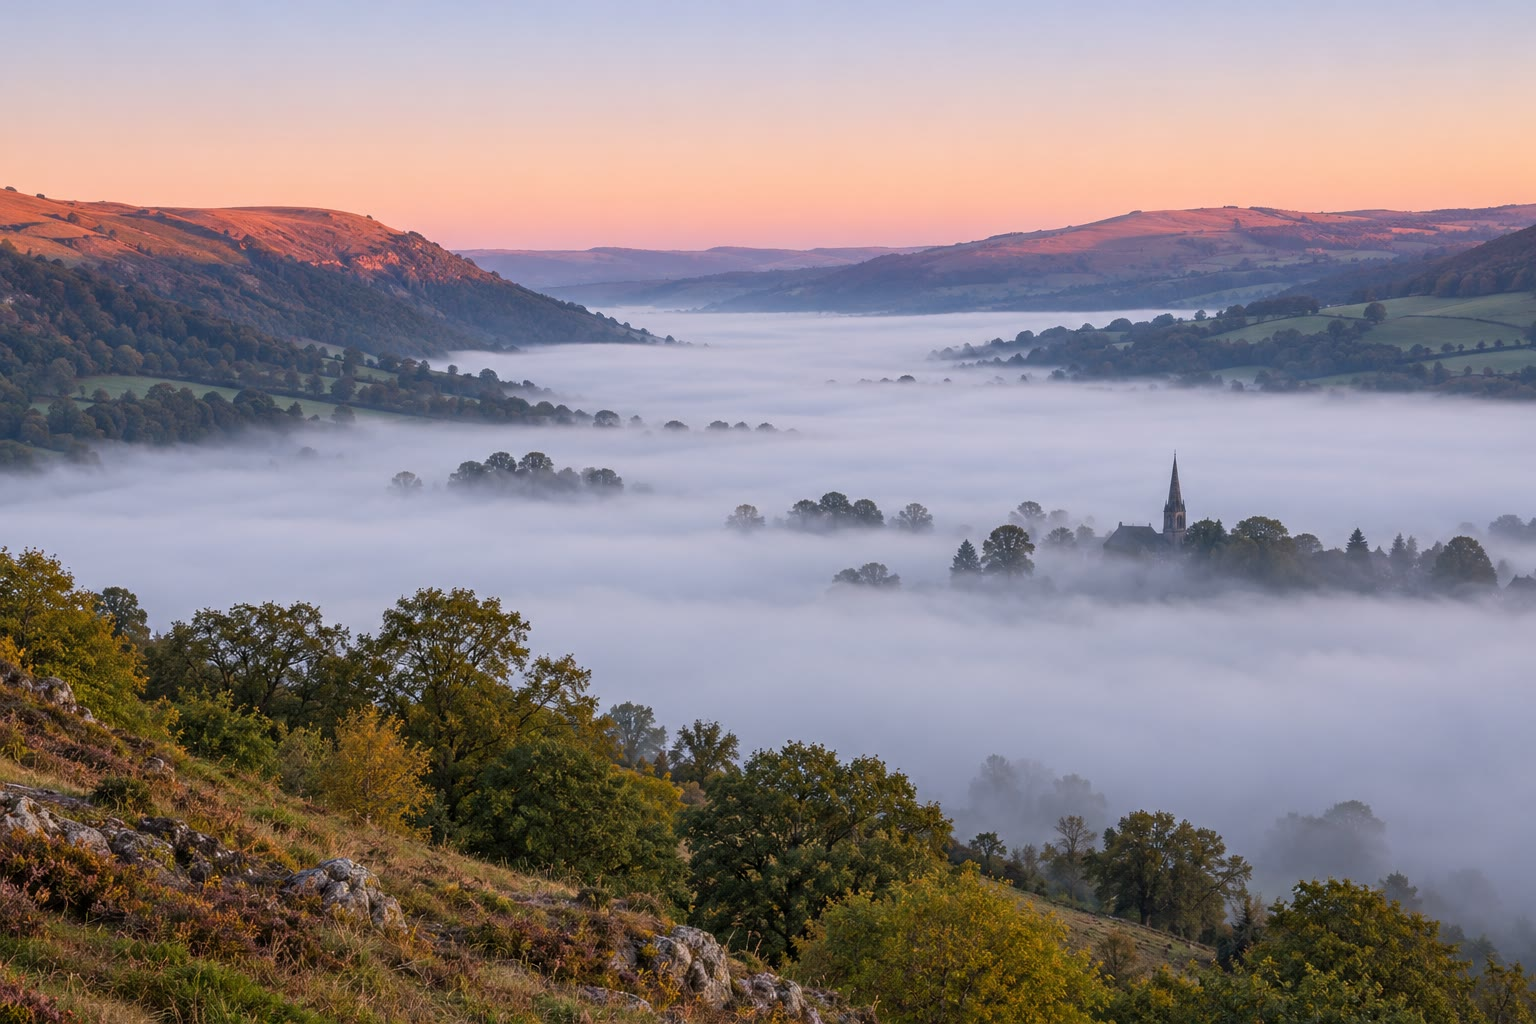
\includegraphics[width=0.75\linewidth]{images/book2/ai/g10-valley-fog.jpg}

{\small ضباب يملأ واديًا عند الفجر. ففي أثناء الليلة الصافية بردت الأرض، وانحدر
الهواء البارد إلى الوادي، وهناك برد إلى ما دون \omterm{def:g10:why-clouds-form:dew-point}{نقطة
نداه}.}
\end{omfigure}

\section{الهواء الصاعد يبرد}

معظم السحب لا تتكون لأن الهواء يلامس شيئًا باردًا، بل لأن الهواء يصعد. فالضغط
ينخفض مع الارتفاع؛ وكتلة الهواء الصاعدة تتمدد، دافعةً الهواء المحيط بها، وتؤخذ
طاقة هذا الشغل من الكتلة نفسها.

\begin{definition}[التبريد الكظمي؛ المعدل الكظمي الجاف]\label{def:g10:why-clouds-form:adiabatic}
\emph{التبريد الكظمي}\index{تبريد كظمي} هو تبرد كتلة هوائية تتمدد دون أن
تتبادل حرارة مع محيطها. والمعدل الذي يبرد به الهواء غير المشبع الصاعد على هذا
النحو هو \emph{المعدل الكظمي
الجاف}\index{معدل كظمي جاف}، القريب من
\qty{9.8}{\degreeCelsius} لكل كيلومتر من الصعود؛ ويسخن الهواء الهابط بالمعدل
نفسه.
\end{definition}

\begin{proposition}[المعدل الكظمي الجاف]\label{prop:g10:why-clouds-form:dry-rate}
\omterm{def:g10:why-clouds-form:adiabatic}{المعدل الكظمي الجاف} هو $g/c_p$، حيث $g = \qty{9.81}{m/s^2}$ و$c_p
\approx \qty{1005}{J.kg^{-1}.K^{-1}}$ هي الطاقة التي تسخّن كيلوغرامًا من الهواء
درجة واحدة تحت ضغط ثابت: $9.81/1005 \approx
\qty{0.0098}{\degreeCelsius/m}$، أي \qty{9.8}{\degreeCelsius/km}.
(نقبله: فبرهانه من شأن كتب الفيزياء.)
\end{proposition}
% ledger: const:gn, const:R, earth:Mmol (c_p of dry air computed as (7/2)R/M in figdata/grade-10/clouds.py)

تنخفض \omterm{def:g10:why-clouds-form:dew-point}{نقطة ندى} الكتلة أيضًا وهي تصعد، لكن ببطء: فمحتواها من الماء يبقى نفسه،
بينما يجعل انخفاض الضغط \omterm{def:g10:why-clouds-form:humidity}{تشبع} البخار أسهل قليلًا. ويعطي الحساب للهواء القريب من
الأرض نحو \qty{1.8}{\degreeCelsius} لكل كيلومتر. فدرجة حرارة الكتلة تقترب إذن من
\omterm{def:g10:why-clouds-form:dew-point}{نقطة نداها} بنحو $9.8 - 1.8 = \qty{8}{\degreeCelsius}$
لكل كيلومتر تصعده.
% ledger: iapws:vapour-pressure (dew-point rate computed in figdata/grade-10/clouds.py)

\begin{definition}[مستوى التكاثف]\label{def:g10:why-clouds-form:condensation-level}
\emph{مستوى التكاثف}\index{مستوى التكاثف} لكتلة هوائية هو الارتفاع الذي تصير
عنده \omterm{def:g10:why-clouds-form:humidity}{مشبعة} وهي تصعد. ويتكاثف الماء فوقه: فمستوى التكاثف هو القاعدة المسطحة للسحب
التي يكوّنها الهواء الصاعد.
\end{definition}

\begin{proposition}[ارتفاع مستوى التكاثف]\label{prop:g10:why-clouds-form:lcl}
الهواء الذي يصعد من الأرض بدرجة حرارة $T$ \omterm{def:g10:why-clouds-form:dew-point}{ونقطة ندى} $T_d$
(بالوحدة \unit{\degreeCelsius}) يصير \omterm{def:g10:why-clouds-form:humidity}{مشبعًا} عند نحو
\[
  z = \frac{T - T_d}{8}\ \text{km} = \qty{125}{m} \times (T - T_d).
\]
\end{proposition}

\begin{proof}
على ارتفاع $z$ (بالكيلومتر) تكون درجة حرارة الكتلة $T - 9.8\,z$ \omterm{def:g10:why-clouds-form:dew-point}{ونقطة نداها}
$T_d - 1.8\,z$. وتصير \omterm{def:g10:why-clouds-form:humidity}{مشبعة} حين تتساويان:
$T - 9.8\,z = T_d - 1.8\,z$، إذن $8\,z = T - T_d$ و$z = (T - T_d)/8$ كيلومتر.
وثُمن الكيلومتر \qty{125}{m}.
\end{proof}

\begin{example}[ركام بعد الظهر]\label{ex:g10:why-clouds-form:base}
% ledger: iapws:vapour-pressure (exact ascent computed in figdata/grade-10/clouds.py: 1.51 km)
بعد ظهر يوم \cref{ex:g10:why-clouds-form:morning}، يكون الهواء عند الأرض في
\qty{28}{\degreeCelsius} \omterm{def:g10:why-clouds-form:dew-point}{ونقطة نداه}
\qty{16}{\degreeCelsius}. فتصير الفقاعات الصاعدة \omterm{def:g10:why-clouds-form:humidity}{مشبعة} عند
$125 \times 12 = \qty{1500}{m}$: فقواعد الركام المسطحة على ارتفاع نحو
\qty{1.5}{km}. أما في الصباح، عند \qty{20}{\degreeCelsius}، فكان الهواء نفسه
سيتكاثف على ارتفاع $125 \times 4 = \qty{500}{m}$ فقط: فقواعد السحب ترتفع على مدى
النهار مع سخونة الأرض.
\end{example}

\section{الهواء المستقر والهواء غير المستقر}

مواصلة الكتلة الصاعدة صعودها تتوقف على الهواء المحيط بها. فالكتلة الأدفأ من
محيطها أخف من الهواء الذي تزيحه فتصعد، كمنطاد الهواء الساخن؛ والكتلة الأبرد من
محيطها تهبط عائدة.

\begin{definition}[الهواء المستقر؛ الهواء غير المستقر]\label{def:g10:why-clouds-form:stability}
يكون الهواء \emph{مستقرًا}\index{هواء مستقر} حين تصير الكتلة المدفوعة نحو الأعلى
أبرد من الهواء المحيط بها، فتهبط عائدة إلى حيث بدأت. ويكون
\emph{غير مستقر}\index{هواء غير مستقر} حين تصير الكتلة أدفأ من الهواء المحيط بها
فتواصل الصعود من تلقاء نفسها.
\end{definition}

تبرد الكتلة الصاعدة \omterm{def:g10:why-clouds-form:adiabatic}{بالمعدل الكظمي الجاف}، \qty{9.8}{\degreeCelsius} لكل
كيلومتر، ما دامت غير مشبعة. فإذا \omterm{def:g10:why-clouds-form:humidity}{تشبعت} بردت ببطء أكبر: لأن التكاثف يحرر \omterm{def:g10:earth-energy-budget:latent-heat}{حرارة
كامنة} في الكتلة. ويعطي الحساب نحو \qty{4.7}{\degreeCelsius} لكل كيلومتر في الهواء
الدافئ قرب الأرض، ونحو \num{5.8} عند \qty{0}{\degreeCelsius}، وأكثر في الهواء
البارد في الأعالي، حيث لا يبقى إلا قليل من الماء ليتكاثف؛ وهذا هو المعدل \omterm{def:g10:why-clouds-form:humidity}{المشبع}.
(وتُستنتج صيغته في المجلدات الجامعية.)
% ledger: nist:water-latent, iapws:vapour-pressure (saturated rates computed in figdata/grade-10/clouds.py)

\begin{method}[هل هذا الهواء مستقر؟]\label{met:g10:why-clouds-form:stable}
\begin{enumerate}
  \item أوجد مدى سرعة انخفاض درجة حرارة الهواء المحيط مع الارتفاع (معدل التناقص
        الحراري البيئي، من سبر بالمنطاد).
  \item قارنه بالمعدل الذي تبرد به الكتلة: المعدل الجاف، نحو
        \qty{9.8}{\degreeCelsius/km}، تحت مستوى تكاثفها؛ والمعدل \omterm{def:g10:why-clouds-form:humidity}{المشبع}، نحو
        \qty{5}{\degreeCelsius/km}، فوقه.
  \item إذا برد المحيط أبطأ من الكتلة، انتهت الكتلة أبرد منه: \omterm{def:g10:why-clouds-form:stability}{فالهواء مستقر}. وإذا
        برد أسرع، انتهت الكتلة أدفأ: \omterm{def:g10:why-clouds-form:stability}{فالهواء غير مستقر}. والطبقة التي \emph{ترتفع}
        فيها درجة الحرارة مع الارتفاع مستقرة جدًا: إذ توقف الهواء الصاعد كغطاء.
\end{enumerate}
\end{method}

مع معدل التناقص المتوسط البالغ نحو \qty{6.5}{\degreeCelsius/km}، يكون الهواء \omterm{def:g10:why-clouds-form:stability}{مستقرًا}
ما دام غير مشبع (فالكتلة تبرد أسرع) \omterm{def:g10:why-clouds-form:stability}{وغير مستقر} متى \omterm{def:g10:why-clouds-form:humidity}{تشبع} (فالكتلة تبرد أبطأ). ويقال
عن مثل هذا الهواء إنه \omterm{def:g10:why-clouds-form:stability}{غير مستقر} شرطيًا: فهو مستقر ما لم يرفعه شيء إلى مستوى
تكاثفه، وعندئذ تنمو السحابة من تلقاء نفسها.

\begin{omfigure}
\begin{tikzpicture}
\begin{axis}[omrecord, width=0.9\linewidth, height=7.6cm, xmin=-30, xmax=36,
  ymin=0, ymax=6, xlabel={\foreignlanguage{arabic}{درجة الحرارة \babelsublr{(\unit{\degreeCelsius})}}}, ylabel={\foreignlanguage{arabic}{الارتفاع \babelsublr{(km)}}},
  xtick={-30,-20,...,30}, ytick={0,1,...,6},
  legend style={at={(0.02,0.98)}, anchor=north west, font=\footnotesize, draw=black!30, fill=white},
  tick label style={font=\small}, label style={font=\small}]
\fill[omDef!10] (axis cs:-30,1.51) rectangle (axis cs:36,3.96);
\addplot[black!60, thick] table[x=T_C, y=z_km] {figdata/out/grade-10-clouds-envA.dat};
\addlegendentry{\foreignlanguage{arabic}{السبر \babelsublr{A}}}
\addplot[omProp!90!black, thick, densely dotted] table[x=T_C, y=z_km] {figdata/out/grade-10-clouds-envB.dat};
\addlegendentry{\foreignlanguage{arabic}{السبر \babelsublr{B}}}
\addplot[omThm!85!black, very thick] table[x=T_C, y=z_km] {figdata/out/grade-10-clouds-parcel.dat};
\addlegendentry{كتلة صاعدة}
\addplot[omMeth!85!black, thick, dashed] table[x=Td_C, y=z_km] {figdata/out/grade-10-clouds-dew.dat};
\addlegendentry{نقطة نداها}
\draw[black!50, dashed] (axis cs:-30,1.51) -- (axis cs:36,1.51);
\node[anchor=south west, font=\footnotesize] at (axis cs:-29.5,1.53) {مستوى التكاثف};
\node[anchor=north east, font=\footnotesize, omDef!80!black] at (axis cs:35.5,3.9) {\foreignlanguage{arabic}{سحابة مع \babelsublr{A}}};
\end{axis}
\end{tikzpicture}

{\small كتلة تصعد من الأرض عند \qty{28}{\degreeCelsius} \omterm{def:g10:why-clouds-form:dew-point}{ونقطة نداها}
\qty{16}{\degreeCelsius} (محسوبة): تبرد بالمعدل الجاف حتى تلاقي درجة حرارتها
\omterm{def:g10:why-clouds-form:dew-point}{نقطة نداها} عند \qty{1.5}{km}، ثم بالمعدل \omterm{def:g10:why-clouds-form:humidity}{المشبع} الأبطأ. وسبران مفترضان: في A،
تكون الكتلة أدفأ من محيطها من \qty{1.5}{km} إلى الطبقة الدافئة قرب
\qty{4}{km}، وينمو ركام بينهما (المنطقة المظللة)؛ وفي B، يُبقي هواء أدفأ فوق الأرض
الكتلةَ أبرد من محيطها في كل مكان: \omterm{def:g10:why-clouds-form:stability}{هواء مستقر}، ولا ركام.}
\end{omfigure}
% ledger: iapws:vapour-pressure, nist:water-latent (parcel computed in figdata/grade-10/clouds.py; soundings invented)

وحين يكون الهواء \omterm{def:g10:why-clouds-form:stability}{مستقرًا} ويُرفع مع ذلك --- فوق جبل، أو على طول جبهة --- تنتشر
السحب المتكونة في طبقات رمادية مسطحة: إنه السحاب الطبقي. وحين يكون \omterm{def:g10:why-clouds-form:stability}{غير مستقر}،
تنتفخ السحب نحو الأعلى في أكوام: إنه الركام؛ وحين يبلغ عدم الاستقرار ارتفاعًا
كافيًا، يصير ركامًا مزنيًا في العواصف الرعدية، تنبسط قممه على شكل سندان حين
تلاقي \omterm{def:g10:why-clouds-form:stability}{الهواء المستقر} جدًا فوق الطبقة الدنيا من الغلاف الجوي.

\begin{omfigure}
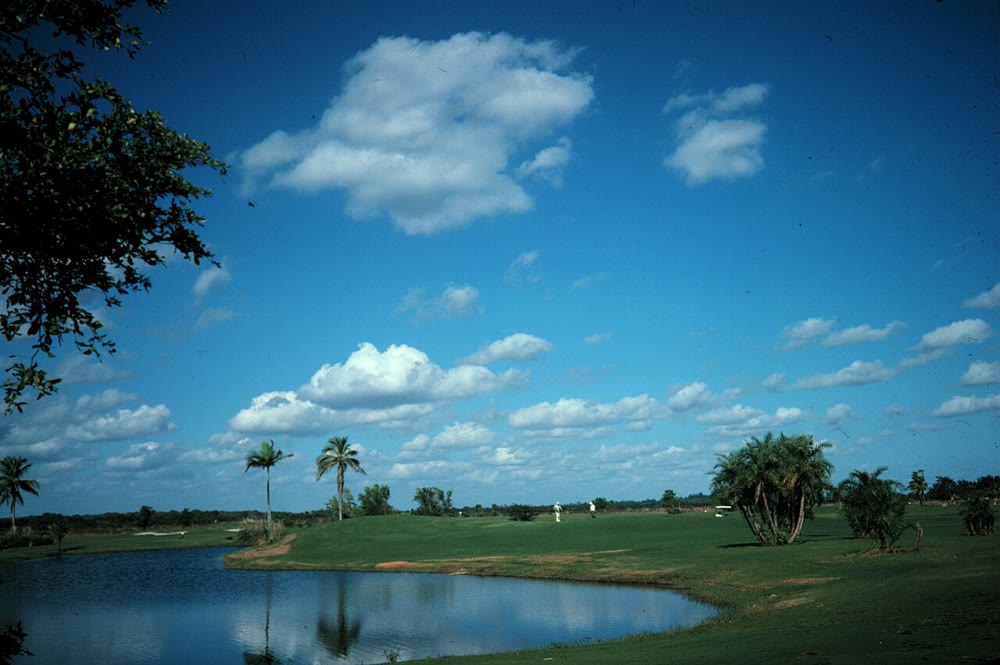
\includegraphics[height=4.5cm]{images/book2/g10-noaa-fair-weather-cumulus.jpg}\hspace{0.6em}%
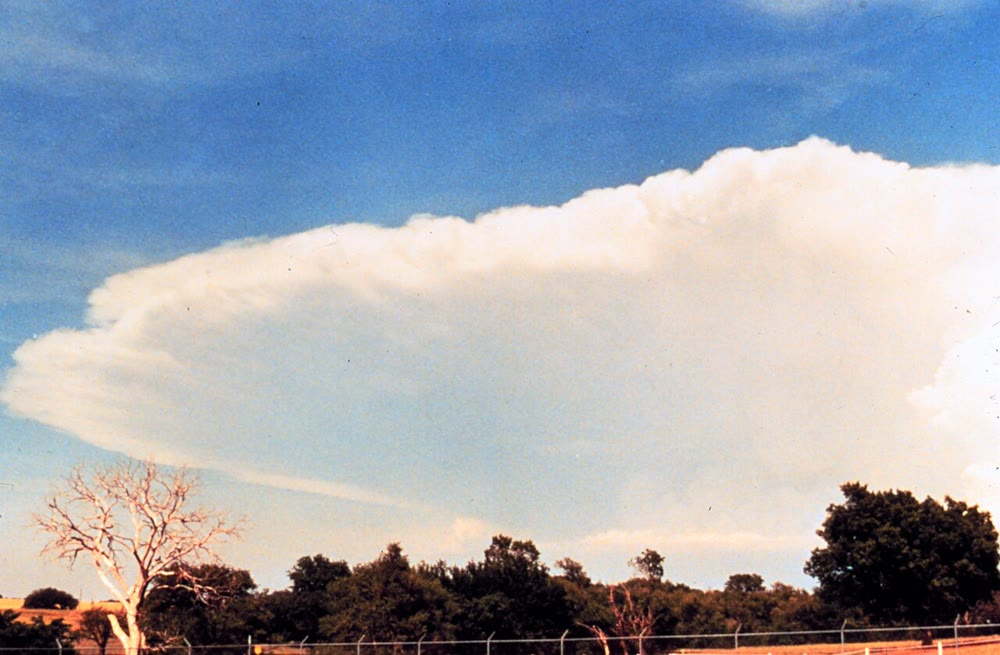
\includegraphics[height=4.5cm]{images/book2/g10-noaa-cumulonimbus-anvil.jpg}

{\small في اليمين: ركام الطقس الصحو فوق فلوريدا، بقواعد مسطحة عند مستوى تكاثفها.
الصورة: رالف ف. كريسغ، الإدارة الوطنية للمحيطات والغلاف الجوي (ملك عام).
في اليسار: سندان ركام مزني في المراحل الأولى من عاصفة.
الصورة: المختبر الوطني للعواصف الشديدة التابع للإدارة الوطنية للمحيطات والغلاف الجوي (ملك عام).}
\end{omfigure}

\section{أربع طرق لرفع الهواء}

يصعد الهواء لأربعة أسباب.
\begin{itemize}
  \item \textbf{التسخين من الأسفل.} في يوم مشمس تسخّن الأرض الهواء الذي فوقها؛
        فتصعد فقاعات من الهواء الدافئ من أسخن البقع. وهي التي تعطي ركام بعد
        الظهر.
  \item \textbf{الجبال.} الريح التي تهب على سلسلة جبلية تُجبر على الصعود على
        سفحها.
  \item \textbf{الجبهات.} حيث تلتقي كتل هوائية دافئة وباردة، يصعد الهواء الدافئ
        الأخف فوق الهواء البارد، أو يندفع الهواء البارد تحته (الكتاب 1،
        الصف 8).
  \item \textbf{التقارب.} حين تلتقي الرياح قرب الأرض، لا يجد الهواء مسلكًا إلا
        إلى الأعلى، كما في حزام الهواء الصاعد قرب خط الاستواء وفي مركز
        المنخفض الجوي.
\end{itemize}

\begin{method}[تتبّع كتلة هوائية فوق جبل]\label{met:g10:why-clouds-form:mountain}
\begin{enumerate}
  \item أوجد \omterm{def:g10:why-clouds-form:condensation-level}{مستوى التكاثف} بقاعدة «\qty{125}{m} لكل درجة»؛ وحتى هذا المستوى تبرد الكتلة
        بمعدل \qty{9.8}{\degreeCelsius/km}.
  \item ومن هناك إلى القمة تبرد بالمعدل \omterm{def:g10:why-clouds-form:humidity}{المشبع}؛ والماء الذي يتكاثف يسقط مطرًا
        أو ثلجًا على الجانب المواجه للريح.
  \item ووراء القمة تهبط الكتلة غير مشبعة: فتسخن بمعدل
        \qty{9.8}{\degreeCelsius/km} طوال نزولها.
\end{enumerate}
\end{method}

\begin{example}[الريح الدافئة الجافة على جانب ظل الريح]\label{ex:g10:why-clouds-form:lee}
% ledger: iapws:vapour-pressure, nist:water-latent (all values computed in figdata/grade-10/clouds.py)
هواء عند مستوى سطح البحر في \qty{20}{\degreeCelsius}، \omterm{def:g10:why-clouds-form:dew-point}{نقطة نداه}
\qty{12}{\degreeCelsius}، تدفعه الريح فوق سلسلة ارتفاعها \qty{2500}{m}. فيصير
\omterm{def:g10:why-clouds-form:humidity}{مشبعًا} عند $125 \times 8 = \qty{1000}{m}$، في نحو
\qty{10}{\degreeCelsius}. ومن هناك إلى القمة يبرد بالمعدل \omterm{def:g10:why-clouds-form:humidity}{المشبع}، حتى نحو
\qty{2}{\degreeCelsius}، ويفقد مطرًا نحو ثلث مائه (من \num{8.7} إلى
\qty{6.0}{g/kg}). وفي نزوله على الجانب الآخر يسخن بالمعدل الجاف على مدى
\qty{2.5}{km}: فيبلغ السهل عند نحو \qty{27}{\degreeCelsius}، أي أدفأ بسبع درجات
مما بدأ به، ورطوبته النسبية نحو \qty{27}{\percent}. وتهب مثل هذه الرياح الدافئة
الجافة على جانب ظل الريح من سلاسل جبلية كثيرة.
\end{example}

\begin{omfigure}
\begin{tikzpicture}[font=\footnotesize, >={Stealth[length=2mm]}]
  \fill[omExo!30] (0,0) -- (3.5,0.3) -- (6,3.0) -- (8.5,0.3) -- (12,0) -- (12,-0.25) -- (0,-0.25) -- cycle;
  \draw[thick, black!70] (0,0) -- (3.5,0.3) -- (6,3.0) -- (8.5,0.3) -- (12,0);
  \draw[black!40, dashed] (0,1.2) -- (4.6,1.2);
  \node[anchor=south west, black!60, align=left] at (0.1,1.22) {مستوى\\\foreignlanguage{arabic}{التكاثف، \babelsublr{\qty{1000}{m}}}};
  \foreach \x in {3.62,3.86,4.1} \draw[omDef!60] (\x,1.2) -- (\x-0.06,{0.3+(\x-0.06-3.5)*1.08+0.04});
  \pic[scale=1.1, transform shape] at (4.6,1.22) {puffycloud};
  \pic[scale=0.9, transform shape] at (5.0,2.2) {puffycloud};
  \draw[->, thick, omDef!80!black] (0.2,0.25) -- (2.8,0.5) .. controls (3.6,0.75) .. (4.4,1.7) -- (5.4,2.9) .. controls (5.8,3.4) and (6.2,3.4) .. (6.6,2.9) -- (7.6,1.7) .. controls (8.4,0.75) .. (9.2,0.5) -- (11.8,0.25);
  \node[anchor=east, align=right] at (3.4,2.15) {\foreignlanguage{arabic}{\babelsublr{\qty{10}{\degreeCelsius}}، مشبع}};
  \node[anchor=south, align=center] at (6.0,3.45) {\foreignlanguage{arabic}{القمة \babelsublr{\qty{2500}{m}}: \babelsublr{\qty{2}{\degreeCelsius}}}};
  \node[anchor=west, align=left] at (7.75,2.1) {يهبط ويسخن\\\foreignlanguage{arabic}{بمعدل \babelsublr{\qty{9.8}{\degreeCelsius/km}}}};
  \node[anchor=north, align=center] at (1.0,-0.3) {\qty{20}{\degreeCelsius}\\\foreignlanguage{arabic}{نقطة الندى \babelsublr{\qty{12}{\degreeCelsius}}}};
  \node[anchor=north, align=center] at (11.0,-0.3) {\qty{27}{\degreeCelsius}\\\foreignlanguage{arabic}{نقطة الندى \babelsublr{\qty{6}{\degreeCelsius}}}};
  \node[anchor=north, black!60] at (4.0,-0.3) {مواجه للريح: مطر};
  \node[anchor=north, black!60] at (8.2,-0.3) {ظل الريح: جفاف};
\end{tikzpicture}

{\small كتلة هوائية تعبر سلسلة جبلية (درجات الحرارة محسوبة؛ والمقياس الرأسي مبالغ
فيه). تبرد بالمعدل الجاف حتى مستوى تكاثفها، وبالمعدل \omterm{def:g10:why-clouds-form:humidity}{المشبع} الأبطأ فوقه، فاقدةً
ماء على شكل مطر، ثم تسخن بالمعدل الجاف طوال نزولها على جانب ظل
الريح.}
\end{omfigure}

\section{من القطيرات إلى المطر والثلج}

لا يتكاثف بخار الماء بسهولة في هواء نقي تمامًا. فالقطيرات تتكون على ذرات دقيقة من
المادة.

\begin{definition}[نواة التكاثف]\label{def:g10:why-clouds-form:nucleus}
\emph{نواة التكاثف}\index{نواة تكاثف} جسيم دقيق عالق في الهواء --- حبة من ملح
البحر، أو غبار، أو دخان، أو سخام --- يتكاثف عليه بخار الماء ليكوّن قطيرة
سحابية.
\end{definition}

يبلغ قطر النواة النموذجية نحو \qty{0.0002}{mm}، والقطيرة السحابية نحو
\qty{0.02}{mm}، وقطرة الرذاذ \qty{0.5}{mm}، وقطرة المطر نحو
\qty{2}{mm}. فقطرة المطر أعرض من القطيرة السحابية مئة مرة، فحجمها أكبر
$100^3$ مرة: مليون قطيرة سحابية تصنع قطرة مطر واحدة. والقطيرات السحابية بالغة
الصغر حتى إن أضعف تيار صاعد يبقيها معلقة؛ ولكي يسقط المطر، يجب أن تكبر القطيرات
مئة ضعف.
% ledger: jpl:drop-sizes

\begin{omfigure}
\begin{tikzpicture}
\begin{axis}[width=0.9\linewidth, height=3.4cm, xmode=log, xmin=1e-4, xmax=10,
  ymin=0, ymax=1, axis y line=none, axis x line*=bottom,
  xlabel={\foreignlanguage{arabic}{القطر \babelsublr{(mm)}، بمقياس لوغاريتمي}}, tick label style={font=\small},
  label style={font=\small}, clip=false]
\addplot[only marks, mark=*, omDef!85!black, mark size=2.5pt] coordinates {(0.0002,0.3) (0.02,0.3) (0.5,0.3) (2,0.3)};
\node[anchor=south, font=\footnotesize, align=center] at (axis cs:0.0002,0.42) {نواة\\تكاثف};
\node[anchor=south, font=\footnotesize, align=center] at (axis cs:0.02,0.42) {قطيرة\\سحابية};
\node[anchor=south, font=\footnotesize, align=center] at (axis cs:0.5,0.42) {رذاذ};
\node[anchor=south, font=\footnotesize, align=center] at (axis cs:2,0.42) {قطرة\\مطر};
\end{axis}
\end{tikzpicture}

{\small الأحجام النموذجية، على مقياس كل خطوة فيه عشرة أضعاف سابقتها: كل جسم أعرض
من سابقه بنحو مئة مرة، باستثناء الرذاذ. البيانات: مختبر الدفع النفاث التابع
لناسا.}
\end{omfigure}

وثمة آليتان تجعلانها تكبر.

\begin{definition}[آلية المطر الدافئ؛ آلية البلورات الجليدية]\label{def:g10:why-clouds-form:rain-processes}
في \emph{آلية المطر الدافئ}\index{آلية المطر الدافئ}، تسقط القطيرات الأكبر في
السحابة أسرع من الصغيرة، فتصطدم بها وتندمج معها، وتكبر وهي تسقط. وفي
\emph{آلية البلورات
الجليدية}\index{آلية البلورات الجليدية}، في الجزء من السحابة الأبرد من
\qty{0}{\degreeCelsius} حيث تختلط بلورات الجليد بقطيرات فائقة التبريد (سائلة
دون \qty{0}{\degreeCelsius})، تكبر البلورات بأخذ البخار الذي تبخره القطيرات؛ ثم
تسقط ندفًا ثلجية، وتنصهر قطرات مطر إذا كان الهواء تحتها دافئًا.
\end{definition}

تعمل \omterm{def:g10:why-clouds-form:rain-processes}{آلية البلورات الجليدية} لأن المحتوى عند \omterm{def:g10:why-clouds-form:humidity}{التشبع} فوق الجليد أدنى منه فوق الماء
السائل عند درجة الحرارة نفسها: فعند
\qty{-10}{\degreeCelsius} يبلغ ضغط بخار \omterm{def:g10:why-clouds-form:humidity}{التشبع} \qty{287}{Pa}
فوق الماء و\qty{260}{Pa} فوق الجليد. فالهواء \omterm{def:g10:why-clouds-form:humidity}{المشبع} بالنسبة إلى القطيرات يحمل
من البخار أكثر بنسبة \qty{10}{\percent} مما يحتمله الجليد: فيتكاثف البخار على
البلورات، وتتبخر القطيرات لتعوّضه.
% ledger: iapws:vapour-pressure, iapws:melt-subl (computed in figdata/grade-10/clouds.py)

\begin{remark}[الحرارة الكامنة تغذي العاصفة]\label{rem:g10:why-clouds-form:latent}
كل كيلوغرام من الماء يتكاثف في سحابة يعطي الهواء نحو
\qty{2.5}{MJ}، وهي \omterm{def:g10:earth-energy-budget:latent-heat}{الحرارة الكامنة} التي أُخذت من البحر أو الأرض حين تبخر
(\cref{ch:g10:earth-energy-budget}). وهذه الحرارة هي ما يجعل المعدل \omterm{def:g10:why-clouds-form:humidity}{المشبع} أبطأ
من المعدل الجاف ويبقي الركام المزني صاعدًا؛ ويتتبعها
\cref{ch:g10:storms-and-cyclones} في أكبر العواصف.
\end{remark}
% ledger: nist:water-latent

\section{تمارين}

استعمل في هذه التمارين المحتويات عند \omterm{def:g10:why-clouds-form:humidity}{التشبع} (بالوحدة \unit{g/kg}، عند ضغط
مستوى سطح البحر) الواردة في الجدول أدناه، والمعدل الجاف
\qty{9.8}{\degreeCelsius/km}، وانخفاضًا \omterm{def:g10:why-clouds-form:dew-point}{لنقطة الندى} قدره \qty{1.8}{\degreeCelsius/km}،
ومعدلًا \omterm{def:g10:why-clouds-form:humidity}{مشبعًا} قدره \qty{5}{\degreeCelsius/km}.
% ledger: iapws:vapour-pressure (table from figdata/out/grade-10-clouds-sat.dat, rounded)

\begin{center}
\small
\begin{tabular}{l*{11}{c}}
\hline
درجة الحرارة (\unit{\degreeCelsius}) & 0 & 4 & 8 & 10 & 12 & 14 & 16 & 20 & 24 & 28 & 30 \\
المحتوى عند \omterm{def:g10:why-clouds-form:humidity}{التشبع} (\unit{g/kg}) & 3.8 & 5.0 & 6.7 & 7.6 & 8.7 & 10.0 & 11.4 & 14.7 & 18.9 & 24.1 & 27.2 \\
\hline
\end{tabular}
\end{center}

\begin{exercise}[$\star$]\label{exo:g10:why-clouds-form:1}
عرّف \omterm{def:g10:why-clouds-form:humidity}{الرطوبة النسبية} للهواء \omterm{def:g10:why-clouds-form:dew-point}{ونقطة نداه}.
\end{exercise}

\begin{exercise}[$\star$]\label{exo:g10:why-clouds-form:2}
أعطِ من الجدول المحتوى عند \omterm{def:g10:why-clouds-form:humidity}{التشبع} عند \num{0} و\num{10}
و\num{20} و\qty{30}{\degreeCelsius}. وبأي عامل تقريبًا يكبر مع كل
احترار بمقدار \qty{10}{\degreeCelsius}؟
\end{exercise}

\begin{exercise}[$\star$]\label{exo:g10:why-clouds-form:3}
هواء عند \qty{24}{\degreeCelsius} يحتوي على \qty{10.0}{g/kg} من بخار الماء.
أوجد رطوبته النسبية \omterm{def:g10:why-clouds-form:dew-point}{ونقطة نداه}.
\end{exercise}

\begin{exercise}[$\star$]\label{exo:g10:why-clouds-form:4}
فسّر لماذا «تتعرّق» كأس الماء المثلج في الصيف، ولماذا لا يحدث ذلك في يوم شتوي
جاف جدًا داخل البيت.
\end{exercise}

\begin{exercise}[$\star$]\label{exo:g10:why-clouds-form:5}
سمِّ الطرق الأربع التي يُجبر بها الهواء على الصعود، مع مثال لكل منها.
\end{exercise}

\begin{exercise}[$\star\star$]\label{exo:g10:why-clouds-form:6}
باستعمال \cref{prop:g10:why-clouds-form:lcl}، أوجد ارتفاع قاعدة السحب لهواء
عند \qty{30}{\degreeCelsius} \omterm{def:g10:why-clouds-form:dew-point}{نقطة نداه}
\qty{18}{\degreeCelsius}، ولهواء عند \qty{22}{\degreeCelsius} \omterm{def:g10:why-clouds-form:dew-point}{نقطة
نداه} \qty{20}{\degreeCelsius}. أي اليومين يُرجح أن يكون رماديًا منخفض السحب؟
\end{exercise}

\begin{exercise}[$\star\star$]\label{exo:g10:why-clouds-form:7}
تغادر كتلة من الهواء غير المشبع الأرض عند \qty{18}{\degreeCelsius}.
ما درجة حرارتها على ارتفاع \qty{1}{km} و\qty{2}{km}، إن بقيت
غير مشبعة؟ وإذا هبطت عائدة من \qty{2}{km}، فعند أي درجة حرارة تبلغ
الأرض؟
\end{exercise}

\begin{exercise}[$\star\star$]\label{exo:g10:why-clouds-form:8}
يُظهر سبر بالمنطاد أن درجة الحرارة تنخفض بمقدار \qty{4}{\degreeCelsius}
لكل كيلومتر. هل \omterm{def:g10:why-clouds-form:stability}{الهواء مستقر} بالنسبة إلى كتلة غير مشبعة؟ وبالنسبة إلى كتلة \omterm{def:g10:why-clouds-form:humidity}{مشبعة}؟
وفي عصر يوم حار، تنخفض درجة الحرارة بمقدار \qty{12}{\degreeCelsius} في
الكيلومتر الأول فوق الأرض: فماذا يحدث لفقاعات الهواء الدافئ؟
\end{exercise}

\begin{exercise}[$\star\star$]\label{exo:g10:why-clouds-form:9}
هواء \omterm{def:g10:why-clouds-form:humidity}{مشبع} عند \qty{20}{\degreeCelsius} يُبرَّد إلى
\qty{10}{\degreeCelsius}. كم غرامًا من الماء يتكاثف لكل كيلوغرام من
الهواء؟ وأين تذهب \omterm{def:g10:earth-energy-budget:latent-heat}{الحرارة الكامنة} المتحررة؟
\end{exercise}

\begin{exercise}[$\star\star$]\label{exo:g10:why-clouds-form:10}
كم قطيرة سحابية قطرها \qty{0.02}{mm} تصنع قطرة رذاذ واحدة
قطرها \qty{0.5}{mm}؟ وقطرة مطر واحدة قطرها \qty{2}{mm}؟
\end{exercise}

\begin{exercise}[$\star\star$]\label{exo:g10:why-clouds-form:11}
فسّر خطوة خطوة لماذا يتكون الضباب في الأودية لا على قمم التلال عند الفجر بعد
ليلة صافية هادئة.
\end{exercise}

\begin{exercise}[$\star\star\star$]\label{exo:g10:why-clouds-form:12}
المعدل الجاف $a$ \omterm{def:g10:why-clouds-form:dew-point}{ونقطة الندى} تنخفض بالمعدل $b$ (كلاهما بالوحدة
\unit{\degreeCelsius/km}). بيّن أن \omterm{def:g10:why-clouds-form:condensation-level}{مستوى التكاثف} يقع عند
$z = (T - T_d)/(a - b)$. وفوق هضبة مرتفعة تنخفض \omterm{def:g10:why-clouds-form:dew-point}{نقطة الندى} بمعدل
\qty{1.7}{\degreeCelsius/km}: فماذا تصير قاعدة «\qty{125}{m} لكل
درجة»؟
\end{exercise}

\begin{exercise}[$\star\star\star$]\label{exo:g10:why-clouds-form:13}
هواء عند مستوى سطح البحر في \qty{15}{\degreeCelsius}، \omterm{def:g10:why-clouds-form:dew-point}{نقطة نداه}
\qty{11}{\degreeCelsius}، يعبر سلسلة ارتفاعها \qty{2000}{m}. باتباع
\cref{met:g10:why-clouds-form:mountain}، أوجد \omterm{def:g10:why-clouds-form:condensation-level}{مستوى التكاثف}، ودرجة
الحرارة عنده، ودرجة الحرارة عند القمة، ودرجة الحرارة التي يبلغ بها الهواء السهل
على الجانب الآخر.
\end{exercise}

\begin{exercise}[$\star\star\star$]\label{exo:g10:why-clouds-form:14}
عند \qty{-20}{\degreeCelsius} يبلغ ضغط بخار \omterm{def:g10:why-clouds-form:humidity}{التشبع}
\qty{126}{Pa} فوق الماء و\qty{103}{Pa} فوق الجليد. بأي نسبة مئوية يكون الهواء
\omterm{def:g10:why-clouds-form:humidity}{المشبع} بالنسبة إلى القطيرات فائق \omterm{def:g10:why-clouds-form:humidity}{التشبع} بالنسبة إلى الجليد؟ قارن بالحالة عند
\qty{-10}{\degreeCelsius}، وقل في أي جزء من السحابة تعمل \omterm{def:g10:why-clouds-form:rain-processes}{آلية البلورات الجليدية}
على أفضل وجه.
\end{exercise}

\begin{exercise}[$\star\star\star$]\label{exo:g10:why-clouds-form:15}
يبرد الهواء المحيط بمعدل \qty{6.5}{\degreeCelsius/km}. تبدأ كتلة هوائية عند
درجة حرارة محيطها نفسها وتصعد \qty{1}{km}. احسب الفرق بين درجة حرارتها ودرجة
حرارة المحيط إن كانت غير مشبعة، ثم إن كانت \omterm{def:g10:why-clouds-form:humidity}{مشبعة}. وفسّر عبارة «\omterm{def:g10:why-clouds-form:stability}{غير مستقر}
شرطيًا».
\end{exercise}

\section{مسألة: عصر يوم صيفي فوق السهل}

\begin{problem}[{مسألة نهاية الأسبوع --- من رطوبة الصباح إلى قاعدة سحب بعد
الظهر}]
\label{pb:g10:why-clouds-form:1}
% ledger: iapws:vapour-pressure, nist:water-latent (all results computed in figdata/grade-10/clouds.py or from the rounded data below; the sounding is sounding A, invented)
فوق سهل واسع، في يوم صيفي، يحتوي الهواء قرب الأرض على
\qty{11.4}{g/kg} من بخار الماء طوال اليوم. وهو عند \qty{20}{\degreeCelsius}
صباحًا و\qty{28}{\degreeCelsius} بعد الظهر. ويعطي سبر بالمنطاد (مثال
مفترض) درجة حرارة الهواء في الأعلى:

\begin{center}
\small
\begin{tabular}{l*{8}{c}}
\hline
الارتفاع (km) & 0 & 0.5 & 1.0 & 1.5 & 2.5 & 3.5 & 3.6 & 4.0 \\
درجة الحرارة (\unit{\degreeCelsius}) & 28.0 & 23.1 & 18.2 & 13.4 & 6.9 & 0.4 & $-0.3$ & 1.2 \\
\hline
\end{tabular}
\end{center}

\noindent استعمل جدول المحتويات عند \omterm{def:g10:why-clouds-form:humidity}{التشبع} والمعدلات المعطاة قبل
التمارين.

\medskip
\noindent\textbf{الجزء الأول --- الرطوبة.}
\begin{enumerate}
  \item أعطِ المحتوى عند \omterm{def:g10:why-clouds-form:humidity}{التشبع} عند \qty{20}{\degreeCelsius}.
  \item احسب \omterm{def:g10:why-clouds-form:humidity}{الرطوبة النسبية} صباحًا.
  \item أوجد \omterm{def:g10:why-clouds-form:dew-point}{نقطة ندى} الهواء.
  \item احسب \omterm{def:g10:why-clouds-form:humidity}{الرطوبة النسبية} بعد الظهر.
  \item هل صار الهواء أجف بعد الظهر؟ فسّر.
\end{enumerate}

\medskip
\noindent\textbf{الجزء الثاني --- الليل والندى.}
\begin{enumerate}[resume]
  \item في أثناء الليل يبرد الهواء قرب الأرض. فعند أي درجة حرارة يبدأ الندى
        بالتكون؟
  \item إذا برد الهواء إلى \qty{12}{\degreeCelsius}، فكم غرامًا من الماء لكل
        كيلوغرام من الهواء قد تكاثف؟
  \item لماذا يتكون الندى على العشب وعلى أسطح السيارات قبل أن يتكون في
        الهواء؟
\end{enumerate}

\medskip
\noindent\textbf{الجزء الثالث --- السبر.}
\begin{enumerate}[resume]
  \item احسب المعدل الذي تنخفض به درجة الحرارة بين
        \num{0} و\qty{1.5}{km}. وقارنه بالمعدل الجاف.
  \item احسبه بين \num{1.5} و\qty{3.5}{km}.
  \item هل الهواء بين \num{1.5} و\qty{3.5}{km} مستقر بالنسبة إلى كتلة
        غير مشبعة؟ وبالنسبة إلى كتلة \omterm{def:g10:why-clouds-form:humidity}{مشبعة}؟
  \item ماذا يحدث بين \num{3.6} و\qty{4.0}{km}؟ وما أثر ذلك في سحابة
        صاعدة؟
\end{enumerate}

\medskip
\noindent\textbf{الجزء الرابع --- قاعدة السحب.}
\begin{enumerate}[resume]
  \item احسب الفرق بين درجة حرارة الهواء \omterm{def:g10:why-clouds-form:dew-point}{ونقطة نداه} عند الأرض بعد
        الظهر.
  \item احسب درجة حرارة فقاعة من هذا الهواء \omterm{def:g10:why-clouds-form:dew-point}{ونقطة نداها} بعد أن تصعد
        \qty{1}{km}، وهي ما زالت غير مشبعة.
  \item بكم تقلّص الفرق بينهما؟ وبأي معدل
        يتقلّص؟
  \item بيّن أن هذا المعدل يعطي قاعدة «\qty{125}{m} لكل درجة».
  \item كم كانت ستكون قاعدة السحب في الصباح؟
  \item فسّر لماذا ترتفع قواعد الركام على مدى النهار.
  \item اكتب المعادلة التي تعبّر عن تساوي درجة حرارة الفقاعة \omterm{def:g10:why-clouds-form:dew-point}{ونقطة نداها} على
        الارتفاع $z$ (بالكيلومتر).
  \item حلّها: على أي ارتفاع تقع قاعدة ركام بعد الظهر؟
\end{enumerate}
\end{problem}
